\documentclass{book}
\usepackage[hidelinks]{hyperref}
\usepackage{titlepic}
\usepackage{titlesec}
\usepackage{graphicx}
\usepackage{caption}
\usepackage{subcaption}
\usepackage{alltt}
\usepackage{fancyhdr}
\usepackage{color}
\usepackage{enumerate}

\DeclareGraphicsExtensions{.pdf,.png,.jpg}
\graphicspath{{./pics/}}

\renewcommand{\labelenumi}{\alph{enumi})}
 
\renewcommand{\headheight}{0.6in}
\setlength{\headwidth}{\textwidth}

\fancyhead[L]{ % left
   \includegraphics[height=0.53in]{mri2}
}
\pagestyle{fancy}

\begin{document}
\title{Exercises: Machine Learning for Bio-Image-Analysis}
\titlepic{
    \includegraphics[width=8cm]{title_image}
    }
\author{Volker Baecker, Cedric Hassen Khodja, Jean-Bernard Fiche\\Montpellier Ressources Imagerie}
\date{22.11.2022}
\maketitle
\tableofcontents
\listoffigures
\chapter{Introduction}

In a scratch assay a gap in a tissue is produced with the tip of a pipette. Images of the tissue are taken in regular time intervals. The relative area of the gap for each time--point is then measured to analyze the speed with which the gap is closing.  

\begin{figure}[!htb]
 \centering
 \includegraphics[width=8cm]{scratch_assay}
 \caption{An image from sratch assay analysis.}
 \label{figure:scratch-assay}
\end{figure}

In this exercise you will try to segment the gap, first using image analysis with FIJI/ImageJ and then using machine learning with Ilastik.

\section{Image Analysis, Features and Scalespace}

Run {\tt FIJI} and open one of the images from the folder {\tt ex01-scratch-assay}.

\begin{figure}[!htb]
 \centering
 \includegraphics[width=8cm]{fiji_open_image}
 \caption{Opening an image in FIJI.}
 \label{figure:fiji-open-image}
\end{figure}

Try to segment the gap and measure its area! Hint: You find some ImageJ commands you might need below.

\subsection{ImageJ commands you might need}

\begin{description}
 \item[Image \textgreater Adjust \textgreater Threshold...] \hfill \\ 
 Create a binary mask from the image.
 \item[Process \textgreater Filters \textgreater Variance...] \hfill \\ Create a new image in which each pixel is replaced with with the variance in a local neighborhood.
 \item[Process \textgreater Find Edges (Sobel filter)] \hfill \\ An edge detector using a combination of convolution filters.
 \item[Process \textgreater Filters \textgreater Gaussian Blur...] \hfill \\ A convolution filter using a Gaussian distribution as kernel. Using a small width of the Gaussian, high frequencies are removed from the image, bigger widths remove lower frequencies. Applying a Gaussian filter with a given width, corresponds to choosing a point in the scale space.
\item[Analyze \textgreater Measure] \hfill \\
Measure the current image or selection. 
\end{description}

The plugin {\tt FeatureJ} provides further features. The selection of a scale, i.e. the application of a Gaussian Blur filter is integrated for the commands of this plugin. The commands of this plugin can be run from a panel that can be opened from {\tt Plugins \textgreater FeatureJ \textgreater FeatureJ Panel}.

\begin{figure}[!htb]
 \centering
 \includegraphics[width=6cm]{featurej_panel}
 \caption{The FeatureJ command-panel.}
 \label{figure:featurej}
\end{figure}

\begin{description}
 \item[Derivatives] \hfill \\ 
 Create an image containing the change (or the change of the change, ...) of the intensities in a given direction.
 \item[Edges] \hfill \\
 A canny edge detector.
 \item[Hessian] \hfill \\
 Creates an image based on the second order partial derivatives of the original image. It can be used to distinguish between plate-like, line-like and blob-like structures.
 \item[Laplacian] \hfill \\
 Creates an image based on the sum of the second order partial derivatives of the image. It is often used for edge and for blob detection. The Laplacian can be implemented as a convolution filter.
 \item[Statistics] \hfill \\
 This command does not create a feature but calculates statistics on an image or a selection. The values calculated can be used to classify objects that have been segmented before.
  \item[Structure] \hfill \\
Creates an image based on the structure tensor which represents the distribution of the gradient directions. It can be used to segment images based on texture.
\end{description}

\section{Machine Learning}

You will now use machine learning to do the segmentation of the gap-area in the scratch assay analysis. 

\begin{enumerate}
\item Start Ilastik and create a new pixel classification project.
\item Add a new (separate) image from the folder {\tt ex01-scratch-assay} to the project.
\begin{figure}[!htb]
 \centering
 \includegraphics[width=8cm]{ilastik}
 \caption{Image import into Ilastik.}
 \label{figure:ilastik}
\end{figure}
\item Adjust the zoom, so that the whole image is visible.
\item Advance to the {\tt Feature Selection} step, open the {\tt Feature Selection Dialog} and select all features on all scales. Also add a new scale of your choice, bigger than the ones initially proposed. We will refine the feature and scale selection later.
\item Close the {\tt Feature Selection Dialog} and click on different features at different scales in the features--list. Which features at which scales do you think are the most useful for the segmentation of the gap? Note the 2 most useful features with their scales:
\begin{verbatim}
Feature 1:


Scale of feature 1:

Feature 2:


Scale of feature 2:

\end{verbatim} 
\item Advance to the {\tt Training} step. Rename the classes for the pixel-classifiction from {\tt Label 1} to {\tt tissue} and from {\tt Label 2} to {\tt gap}. Change the colors of the classes from yellow and blue to red and green.

\item Select the {\tt tissue} class and draw 3 or 4 strokes on the tissue using the brush--tool. Then select the {\tt gap} class and draw 3 or 4 strokes in the gap. Press the {\tt Live Update} button to see the result of the segmentation.

\item If necessary add more strokes for the two classes with the brush--tool or remove strokes using the eraser--tool. The segmentation will be updated immediately as long as the {\tt Live Update} is active.

\item Deactivate the {\tt Live Update} and advance to the {\tt Prediction Export}. Export the segmentation into a {\tt .tiff}--file. You need to select the right {\tt Source} and the right image file-format from the {\tt Choose Export Image Settings} dialog. Then press the {\tt Export All}--button.

\item Open the exported segmentation--image with {\tt Fiji}. The values in the image correspond to the indexes of the classes. In this case they are 1 and 2. Use the threshold-adjuster to create a mask. Run the {\tt fill-holes} command. Use the particle--analyzer to add a selection of the gap to the {\tt roi-manager} and measure the surface of the gap.
\begin{verbatim}
Name of the image:

area of the gap [pixel]: 
\end{verbatim}
\item Go back to {\tt Ilastik} and advance to the {\tt Batch Processing} step. Select some of the images not yet processed, from the folder {\tt ex01-scratch-assay}. Run the segmentation on the input files and control the results with {\tt Fiji}.

\item Open a segmentation--result, create a {\tt ROI} from the selection and display it on the original input image. How good is the segmentation? Does it correctly reflect the borders of the gap/tissue?
\begin{figure}[!htb]
 \centering
 \includegraphics[width=8cm]{wound_healing_result}
 \caption{The ROI of the segmentation displayed on the input image.}
 \label{figure:ilastik-segmentation-result}
\end{figure}

\end{enumerate}
\chapter{Clustering}

In the exercises in this chapter you will first use a visualization of the k-means clustering that helps to understand how it works. You will then apply the k-means clustering as a machine learning method to segment plants based on their color and than on features of the scratch-assay-images.

\section{K-means clustering}

Open the file {\tt Visualizing K-Means Clustering.html} from the folder {\tt 01-k-means-visualization}. The applet allows you to see the k-means clustering at work. You can select different strategies for the initial mean-values and different data--sets. You can follow the k-means algorithm step by step. 

Run the k-means algorithm with different initialization strategies and on different data--sets and answer the following questions.

\begin{enumerate}
\item What influence do you think the selection of the initial mean values has on the clustering result ?
\begin{verbatim}







\end{verbatim}
\item Does the k-means algorithm always converge, i.e. does it always come to a point where further iterations do not change the result anymore?
\begin{verbatim}


\end{verbatim}
\item Is the result of the clustering always the same, no matter what the choice of the initial means is?
\begin{verbatim}


\end{verbatim}
\item Does the k-means clustering work as expected on the {\tt Smiley Face} data--set? What is the reason it does or does not work as expected?
\begin{verbatim}









\end{verbatim}
\end{enumerate}

\section{Using K-means clustering for color segmentation}

Images of Arabidopsis thaliana are taken in regular intervals. The aim is to measure the speed with which the area of the rosette of leaves augments under different conditions and treatments. You will use k-means clustering to segment the rosettes of the plants. You will create a color-stack using an appropriate color-space (RGB, HSB or Lab) and use the {\tt k-means segmentation} tool. 

\begin{figure}[!htb]
 \centering
 \includegraphics[width=8cm]{arabidopsis}
 \caption{Arabidopsis plant at 3 different stages.}
 \label{figure:arabidopsis}
\end{figure}

\begin{enumerate}
\item Run {\tt FIJI} and open one of the images from the folder {\tt 03 - plants}. Convert the image to a color stack using one of the commands {\tt RGB Stack}, {\tt HSB Stack} or {\tt Lab Stack} from the menu {\tt Image>Type}.  Run the {\tt k-means segmentation} tool from the menu {\tt Plugins>k-means experiment>k-means segmentation}.
\begin{figure}[!htb]
 \centering
 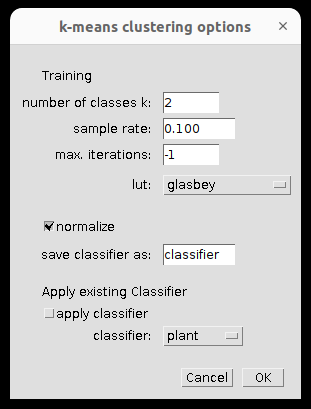
\includegraphics[width=4cm]{color_clustering}
 \caption{The options of the k-means segmentation command.}
 \label{figure:color_clustering}
\end{figure}
\item How many clusters do you think are appropriate? 
\begin{verbatim}
Number of clusters:

\end{verbatim}
Configure the k-means segmentation to use the number of clusters you have decided to use and run it on the stack. The value of a pixel in the result image corresponds to the cluster to which the pixel belongs. 

What is the class of the color values belonging to the plant?
\begin{verbatim}
Class of plant:

\end{verbatim}
What is the class of the color values belonging to the small red reference object in the form of a ball?
\begin{verbatim}
Class of reference object:

\end{verbatim}

\item Create a selection (roi) from the result of the pixel classification and display it on the original input image. Use the commands {\tt select label(s)} and {\tt Keep largest region} to isolate the target label. Then open the threshold adjuster (shift-t) and run the command {\tt create selection}. Transfer the selection to the original input image (restore selection or use the roi-manager). How good is the selection? Measure the area of the surface of the plant.
\begin{verbatim}
Area of the plant:

\end{verbatim}
\item Check the log--window. The clustering algorithm has written the k mean-vectors into the log. What are their values?
\begin{verbatim}
k mean vectors:




\end{verbatim}

\item Apply the saved k-means classifier on a different image from the plant-series.
\end{enumerate}

\section{Using K-means clustering on other features}

We can use the k-means clustering not only with colors but also with other features. 

\begin{enumerate}
\item Open an image from {\tt scratch-assay}-folder. Create two or three feature images from the input image for example by using FeatureJ. Use appropriate scales when creating the features. Use {\tt Image>Color>Merge Channels...} to create a stack of the feature images. Run the k-means clustering on the stack. What is the area of the gap?
\begin{verbatim}
Area of the gap:

\end{verbatim}

\end{enumerate}


\bibliographystyle{plain}
\bibliography{exercises}
\end{document}